\chapter{Introduction}\label{ch:intro}
%% Shift to social media
% Consumption
Modern media and news consumption is shifting from traditional outlets to social media and mobile devices.
People receive local and global news perceived relevant to their group on their social media feed.
The ease of reaching a global audience by an individual with a smartphone diminishes the role of an expert curator handling incoming information.
As such, news is not bound to expert opinion or an editorial news desk anymore.
According to Reuters Institute's Digital News Report 2016, young people in particular are shifting to social media as their number one source \cite{reuters_social_media}, shown in the age distribution graph, Figure \ref{fig:reuters-news-sources-ages}.
\begin{figure}[H]
	\centering
	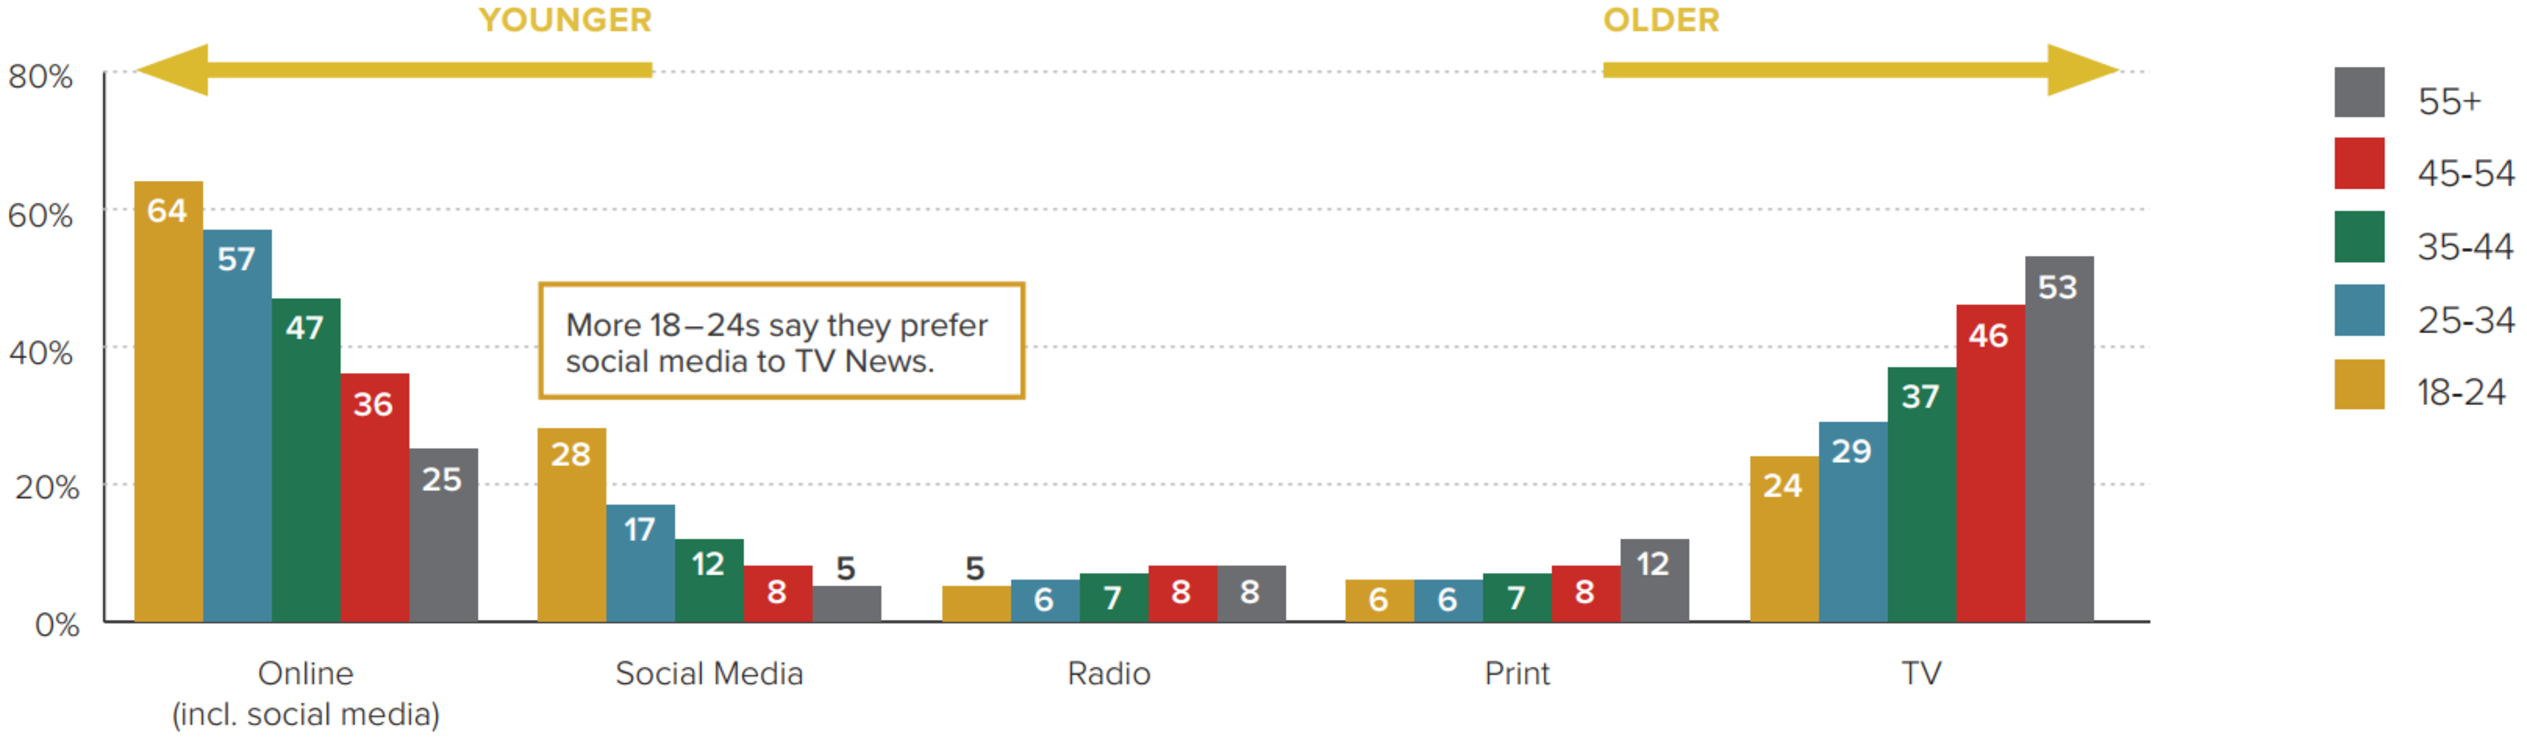
\includegraphics[width=\textwidth]{reuters-news-sources-ages}
	\caption{Main news sources split by age \cite{reuters_social_media}}
	\label{fig:reuters-news-sources-ages}
\end{figure}
%% Rise of the smartphone
% Production
The mobile devices on which news and modern media are consumed are also capable of news production.
The capabilities and versatility of smartphones in particular enable them to be used for both production and consumption.
% Distribution
Most smartphones have one or more cameras to record multi-media content that can be shared immediately from the device.
% Ubiquity
A smartphone also has the unique property of being a ubiquitous device that is highly mobile and extremely connectable.
Figure \ref{fig:smartphone-sales} shows that, world-wide, 1.4 billion smartphones were sold to end-users last year, and shows a considerable growth in the past five years.
%Especially in areas without traditional infrastructure they are ubiquitous.
\begin{figure}[H]
	\centering
	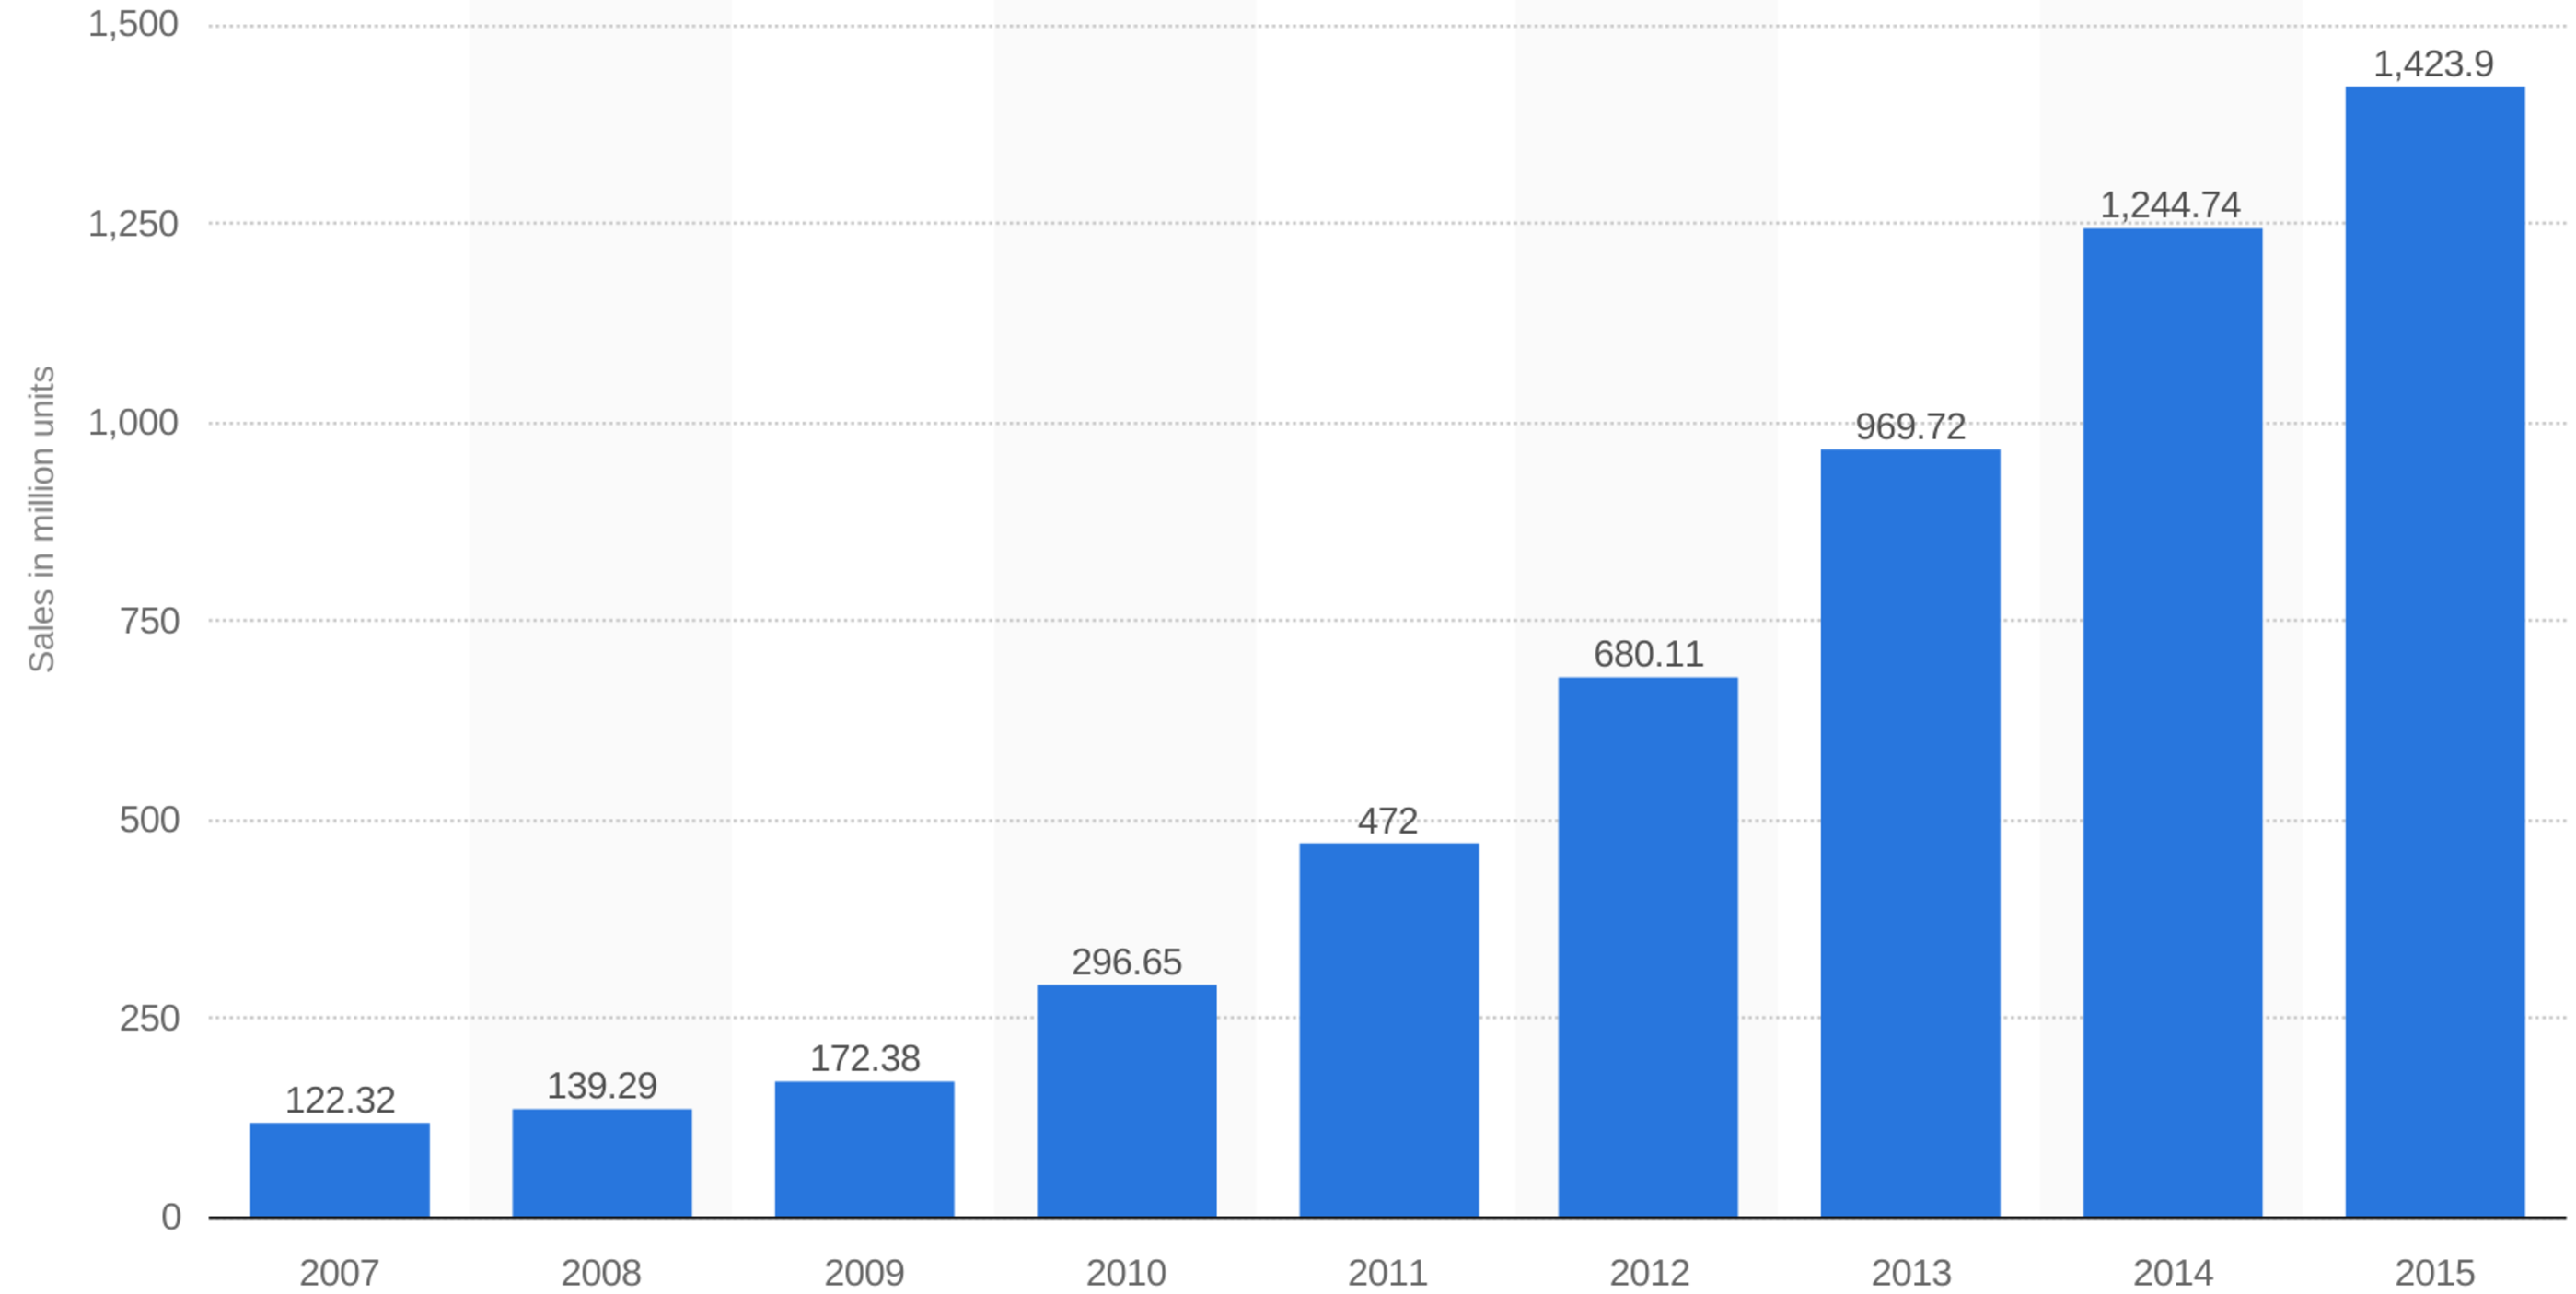
\includegraphics[width=.75\textwidth]{smartphone-sales}
	\caption{Number of smartphones sold to end users worldwide from 2007 to 2015 (in million units) \cite{smartphone-sales}}
	\label{fig:smartphone-sales}
\end{figure}
Eye-witnesses often have smartphones at hand to immediately record an event with and post it on social media.
No news desk or professional equipment is necessary to relay news directly from eye-witnesses to the masses anymore.
The users themselves are turning from con-sumers into pro-sumers \cite{news_crowd}.

Unfortunately, the Internet is censored in some parts of the world, limiting access to news and global opinion online.
Invasion of privacy by large scale monitoring is grave cause for concern \cite{nsa_privacy}.
However, censorship and large scale monitoring on the Internet are problems that can be battled with decentralized solutions \cite{pouwelse2012censorshipfree}.


%% Communication during crisis
In crisis situations, like natural disaster or unrest, people need to communicate and coordinate their efforts to restore safety.
In this context the smartphone becomes particularly important because it is often carried on person and provides connectability.
In the wake of recent calamities, people could mark themselves as safe on social media \cite{fb-safety-check}, effectively broadcasting that information to all their family and friends on social media instead of contacting them one by one or not at all due to congestion in the communication channels.
However, several natural disasters have taken out the necessary infrastructure on numerous occasions for a prolonged period of time \cite{renesys2005katrina}.
Therefore we require a distributed solution using smartphones, that does not require infrastructure.



Tribler is a fully decentralized video-on-demand system. \cite{TriblerOverviewJournal, tribler2014play, tribler-anon-hd}
It is autonomous, attack-resilient and self-organizing. \cite{votecast, tribler-gossip}
It uses network overlays called communities to offer features like keyword search and managing contributions to channels for discover-ability of content.
It offers privacy through layered encrypted tunnels similar to the TOR network.\cite{tor_bittorrent, tribler2014at3, dingledine2004tor, dingledine2006design}

The autonomous, attack-resilient and self-organizing properties of Tribler make it an interesting candidate for handling use scenarios of rapid media dissemination without dependency on centralized infrastructure, and with preservation of anonymity.
However, so far Tribler only supports desktop and server versions of Linux, Mac and Windows.
In order to realize the mobile media dissemination use cases as mentioned above, it will be necessary to enable Tribler on mobile devices, which however may be resource limited.



In this thesis, the first prototype is presented that has all Tribler functionality fully enabled on mobile devices.
The two following research questions are answered in this work:
\begin{enumerate}
	%How to create a \emph{self-organising} \emph{video-on-demand} platform that is \emph{attack-resilient} and can \emph{operate autonomously} on a \emph{mobile device}?
	\item How feasible is it to run all Tribler functionality on mobile devices? % to defeat or mitigate large scale monitoring and censorship?
	\item Given the constraints and unique abilities of mobile devices, what functionality of Tribler can be added or enhanced?
\end{enumerate}
A prototype is built for Android OS, since Android currently dominates the smartphone market.
Its modular architecture is specifically designed for portability and maintainability.

% Research Limitations
% Project scope
% broad / narrow scope, scope of other system()s)
% sub-problems
% ultimate high-level goal
% Software development / technical aspect only
% Not policy making, organisational perspective, decision making, normative, ethical,
% Time limit of 9 months

The remainder of this thesis is organized as follows.
The problem of media dissemination under adversary conditions is described by Chapter \ref{ch:problem_desc}.
Tribler's functionality is described in Chapter \ref{ch:tribler}, as well as a short discussion of the specific opportunities and challenges that mobile devices bring with them.
These lead to the requirements, which are listed in Chapter \ref{ch:design}, followed by a fitting system architecture design.
An implementation for Android, that satisfies the design requirements, is presented in Chapter \ref{ch:implementation}.
This implementation is then used to analyze the performance of Tribler on smartphones and tablets, and resulting performance measurements are presented and discussed in Chapter \ref{ch:results}.
Finally, the research questions are answered based on the results of the experiments in Chapter \ref{ch:conclusions}, and suggestions are made for future research, based on this work.

